\appendix{Представление графического материала}

Графический материал, выполненный на отдельных листах,
изображен на рисунках А.1--А.\arabic{числоПлакатов}.
\setcounter{числоПлакатов}{0}

\renewcommand{\thefigure}{А.\arabic{figure}} % шаблон номера для плакатов

\begin{landscape}

\begin{плакат}
	\centering
    
\includegraphics[width=0.84\linewidth]{main.png}
  	\заголовок{Сведения о ВКРБ}
    \label{pl1:image}      
\end{плакат}

\begin{плакат}
    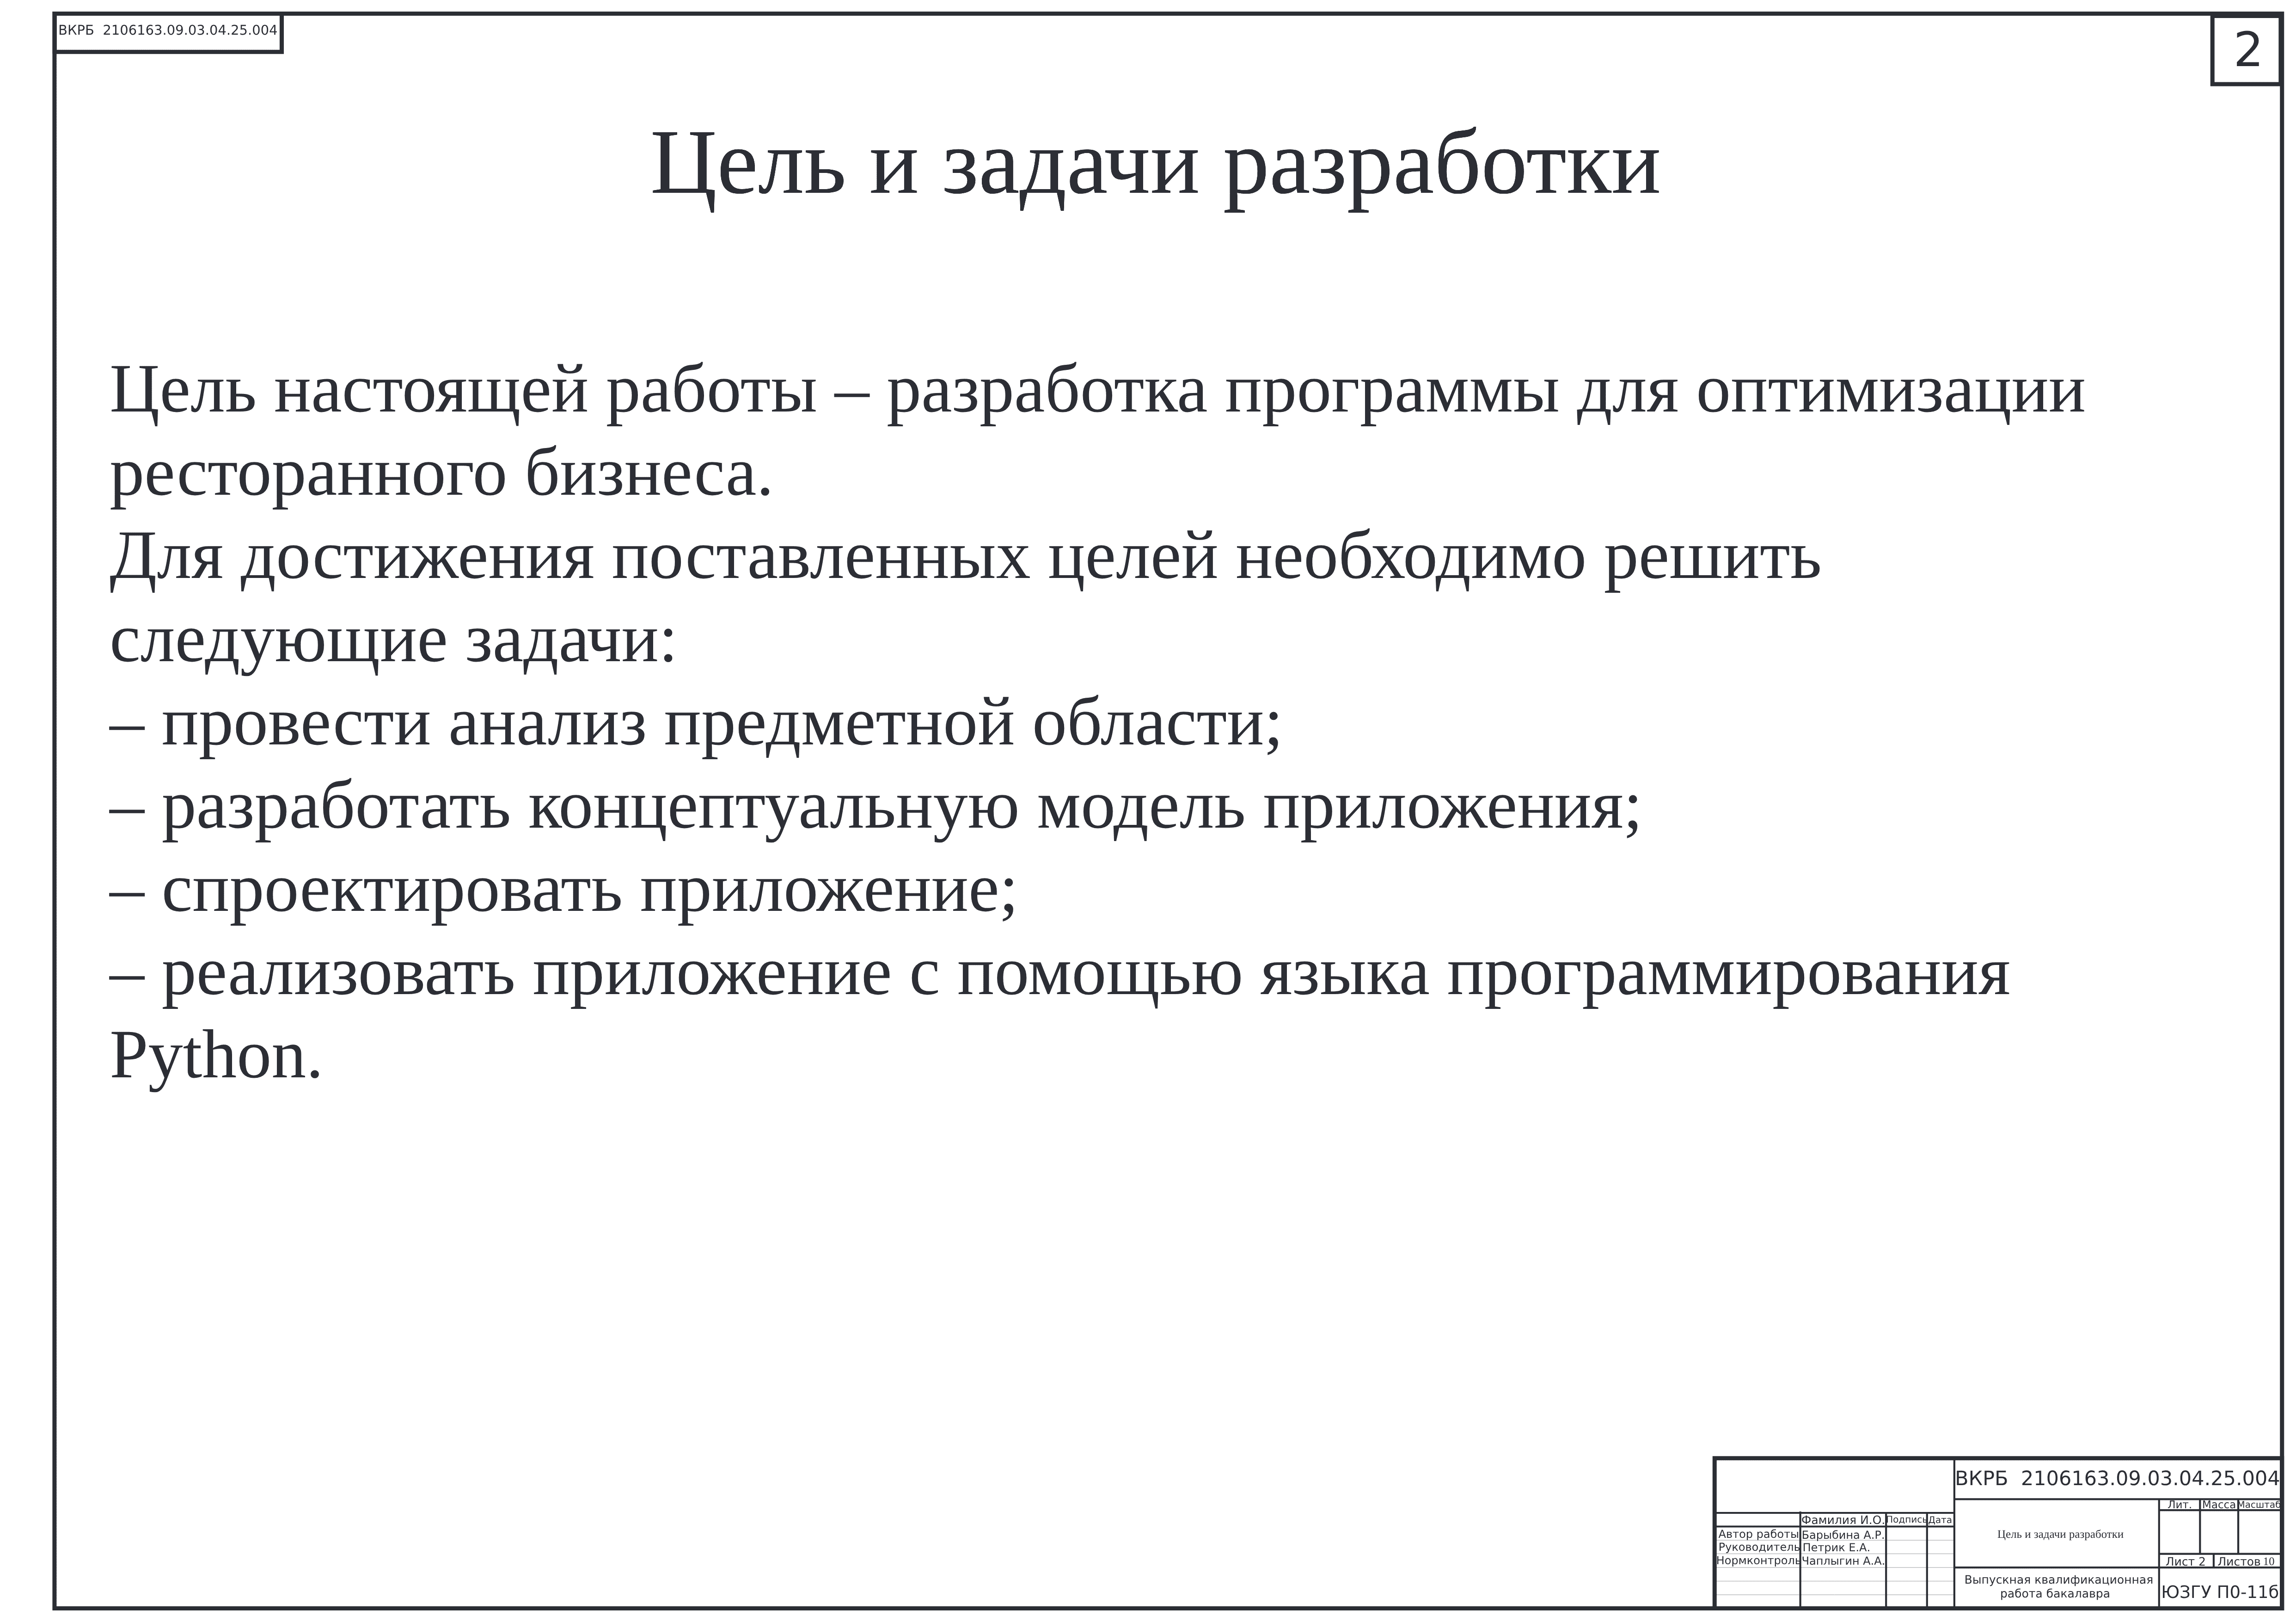
\includegraphics[width=0.84\linewidth]{zadachi.png}
    \заголовок{Цель и задачи разработки}
    \label{pl2:image}      
\end{плакат}

\begin{плакат}
	
\includegraphics[width=0.84\linewidth]{plakat.png}
	\заголовок{Компоненты программно-информационной системы управления ресторанным бизнесом}
	\label{pl3:image}      
\end{плакат}

\begin{плакат}
    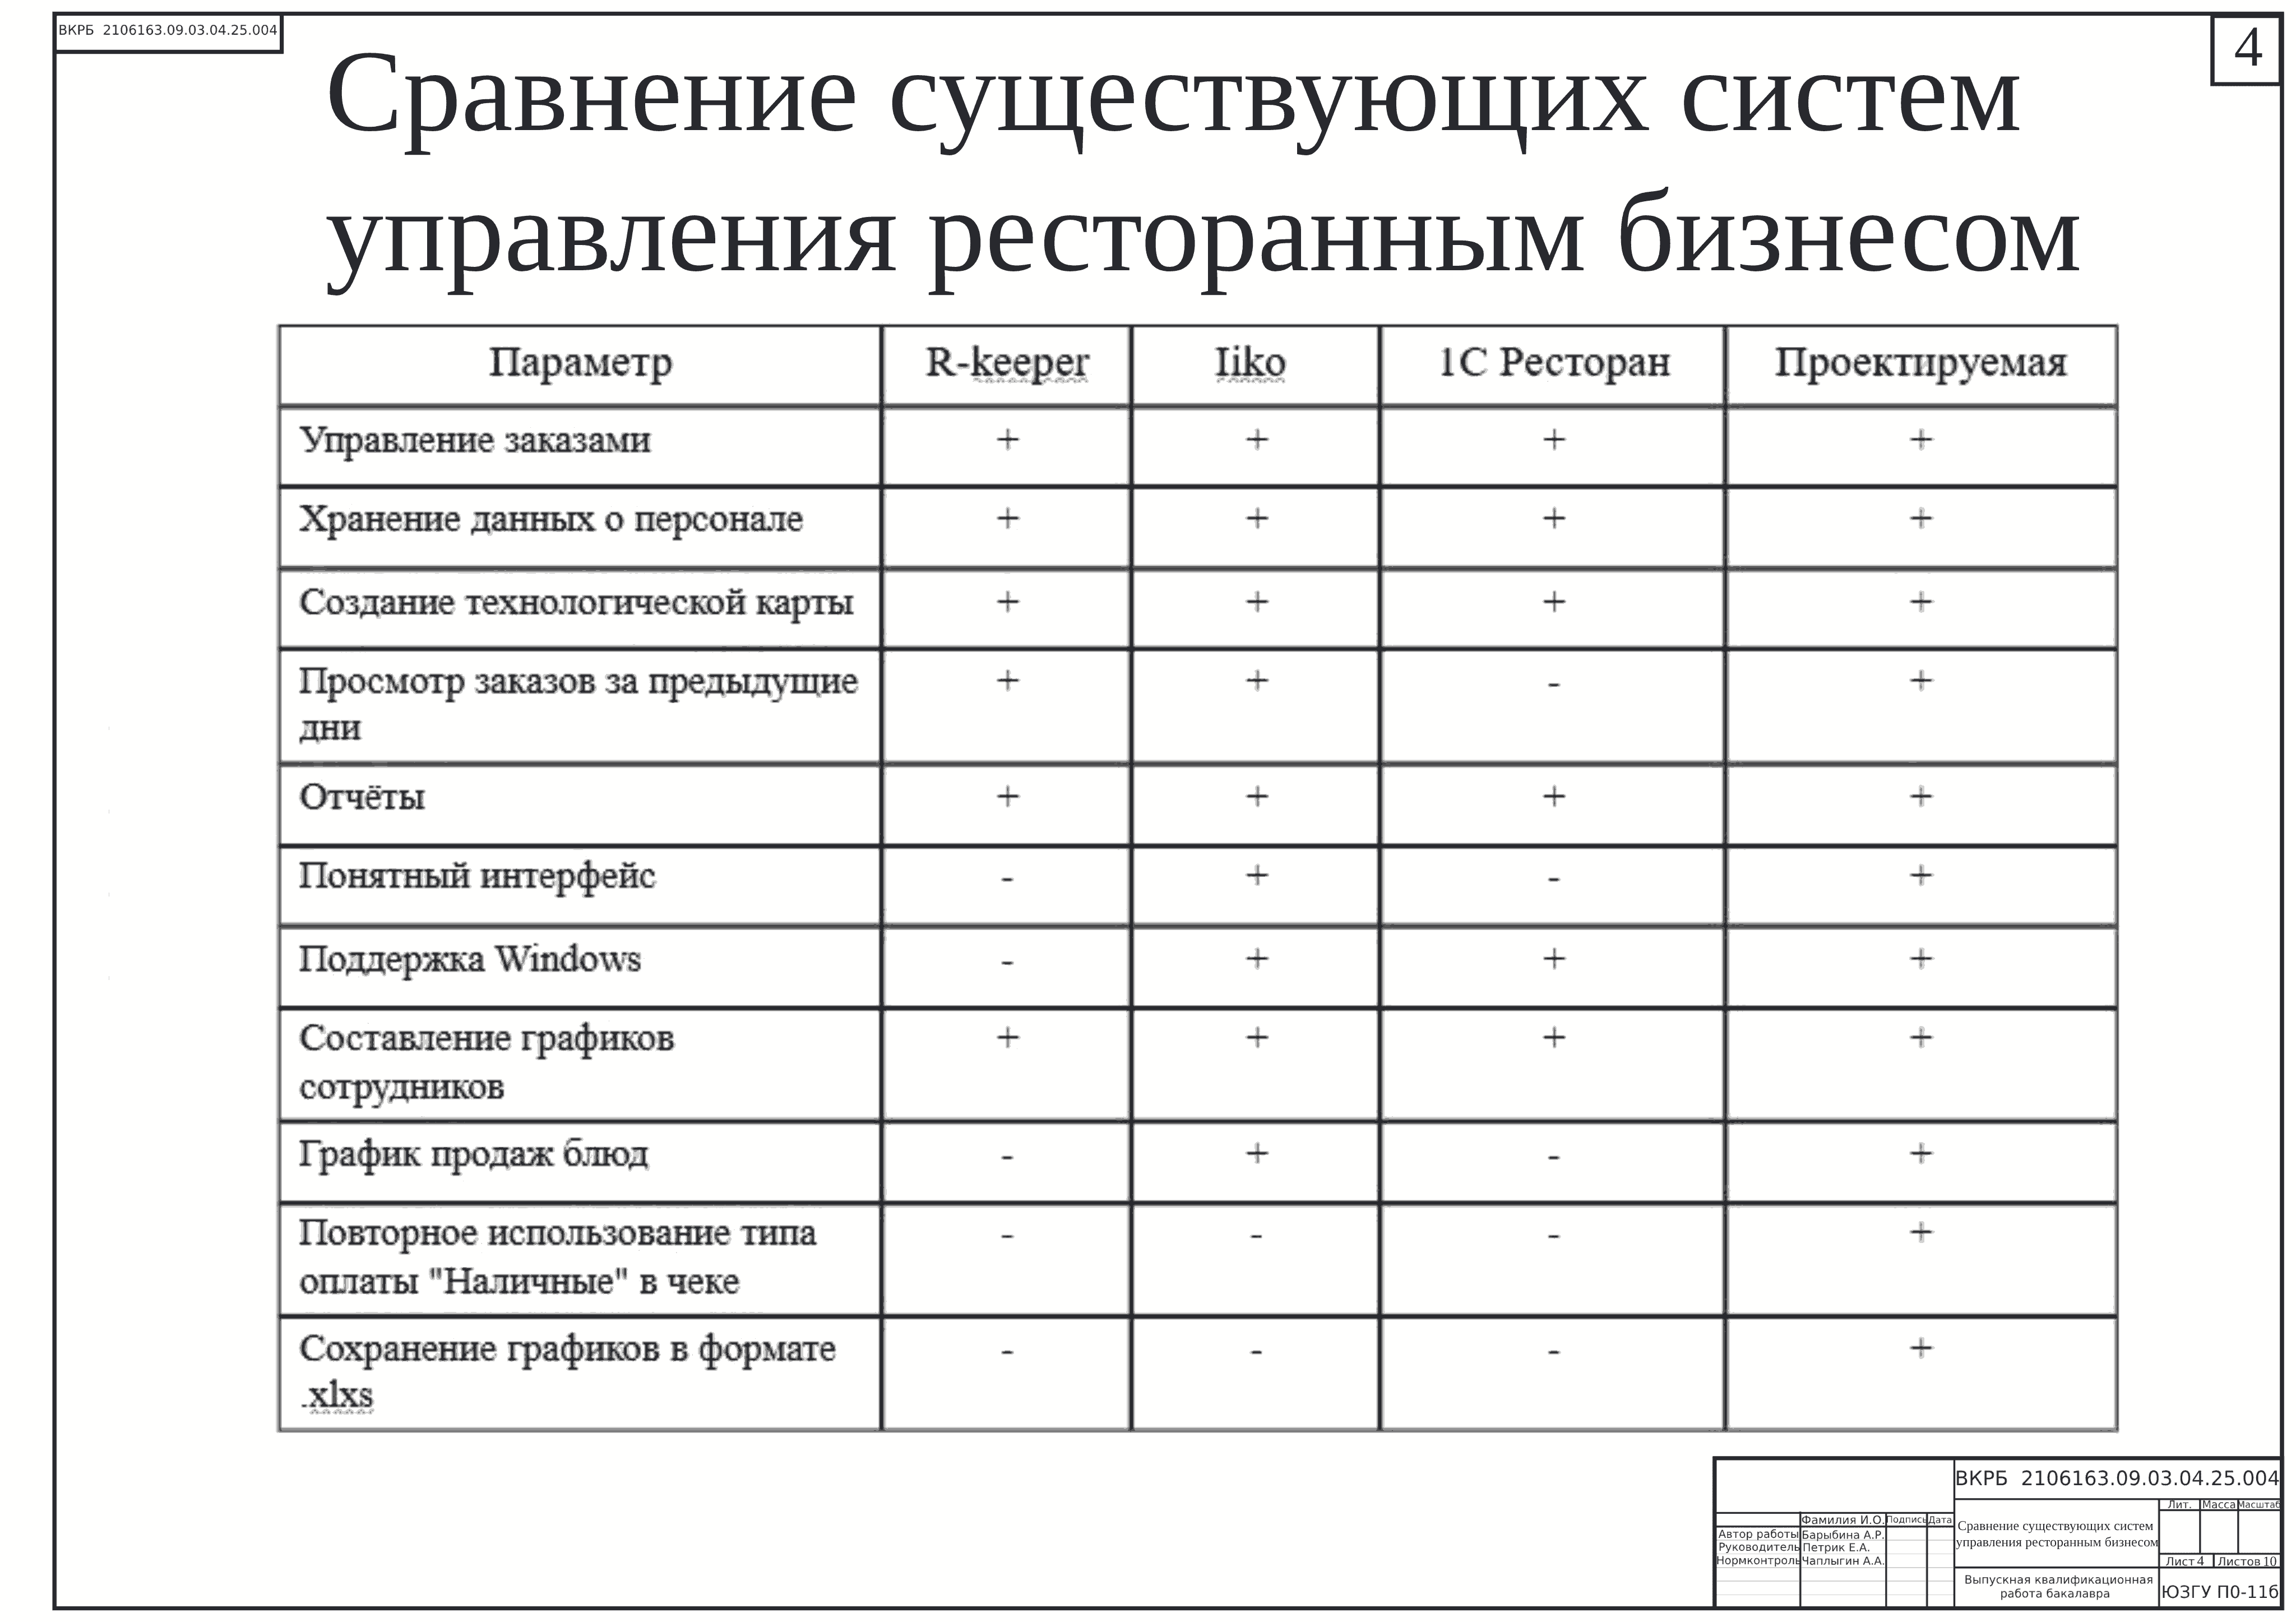
\includegraphics[width=0.84\linewidth]{differentsys.png}
    \заголовок{Сравнение существующих систем управления бизнесом с проектируемой}
    \label{pl4:image}      
\end{плакат}

\begin{плакат}
	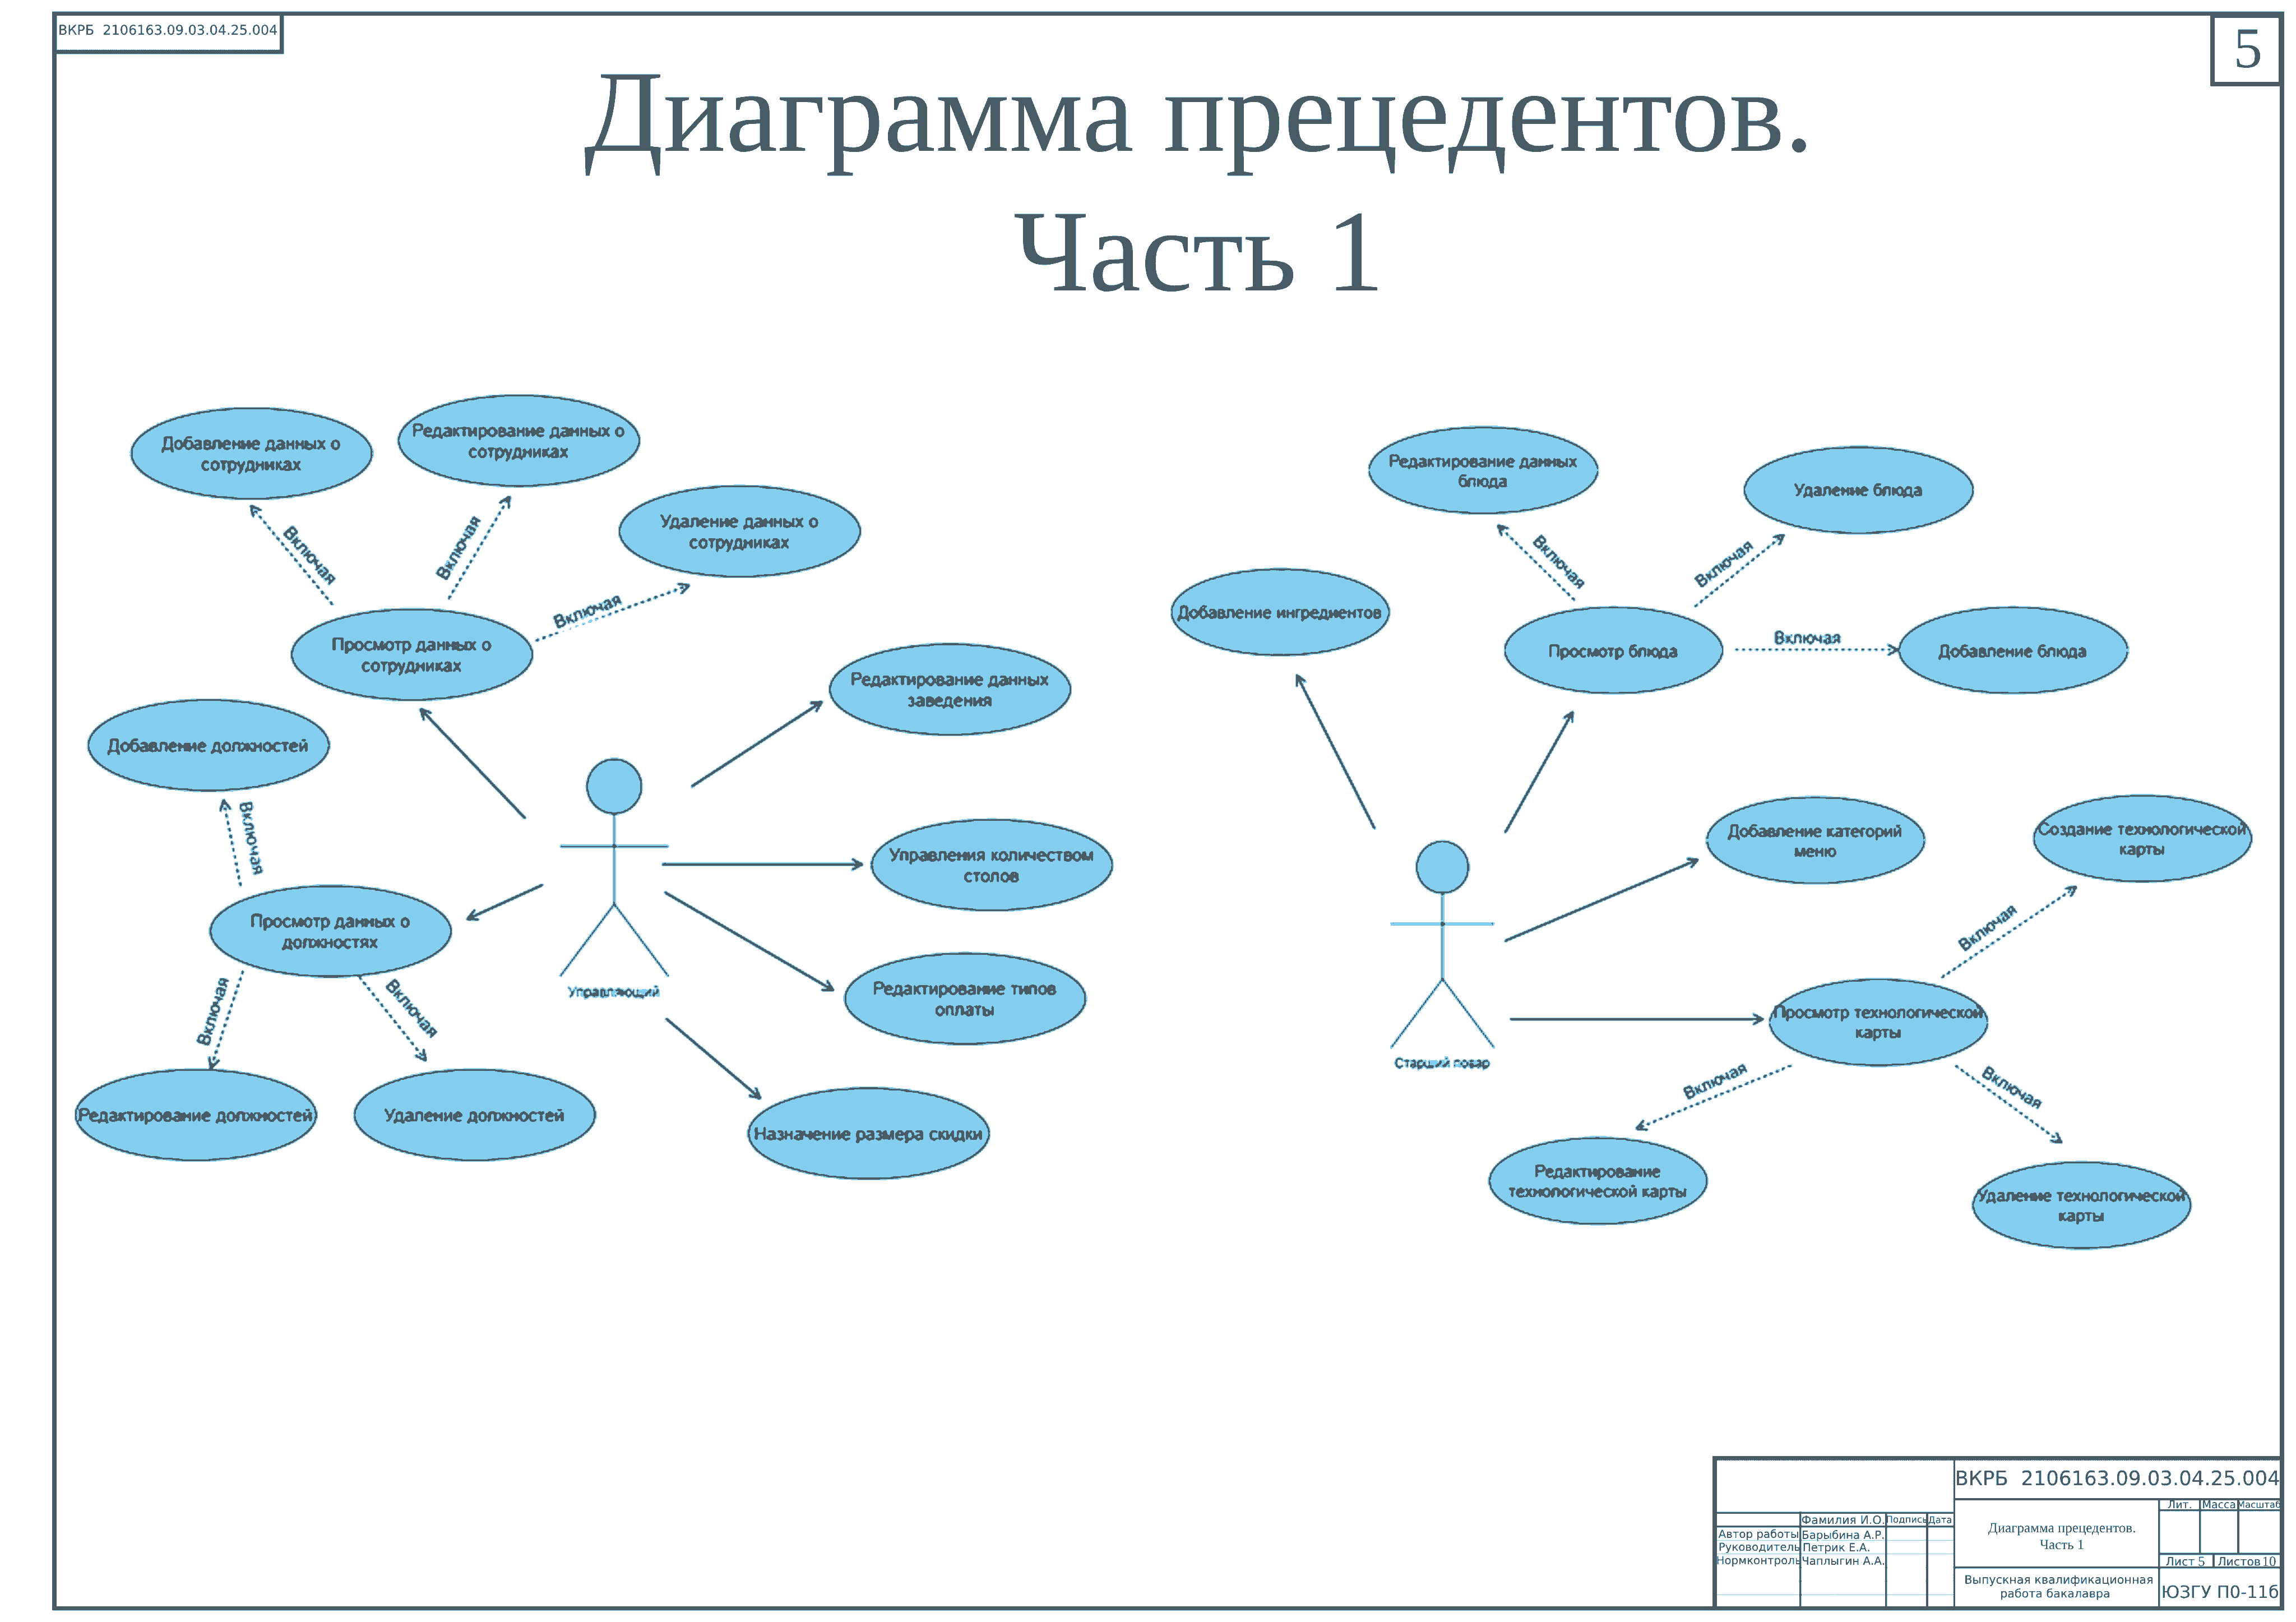
\includegraphics[width=0.84\linewidth]{precedent1.png}
	\заголовок{Диаграмма прецедентов. Часть 1}
	\label{pl5:image}      
\end{плакат}

\begin{плакат}
	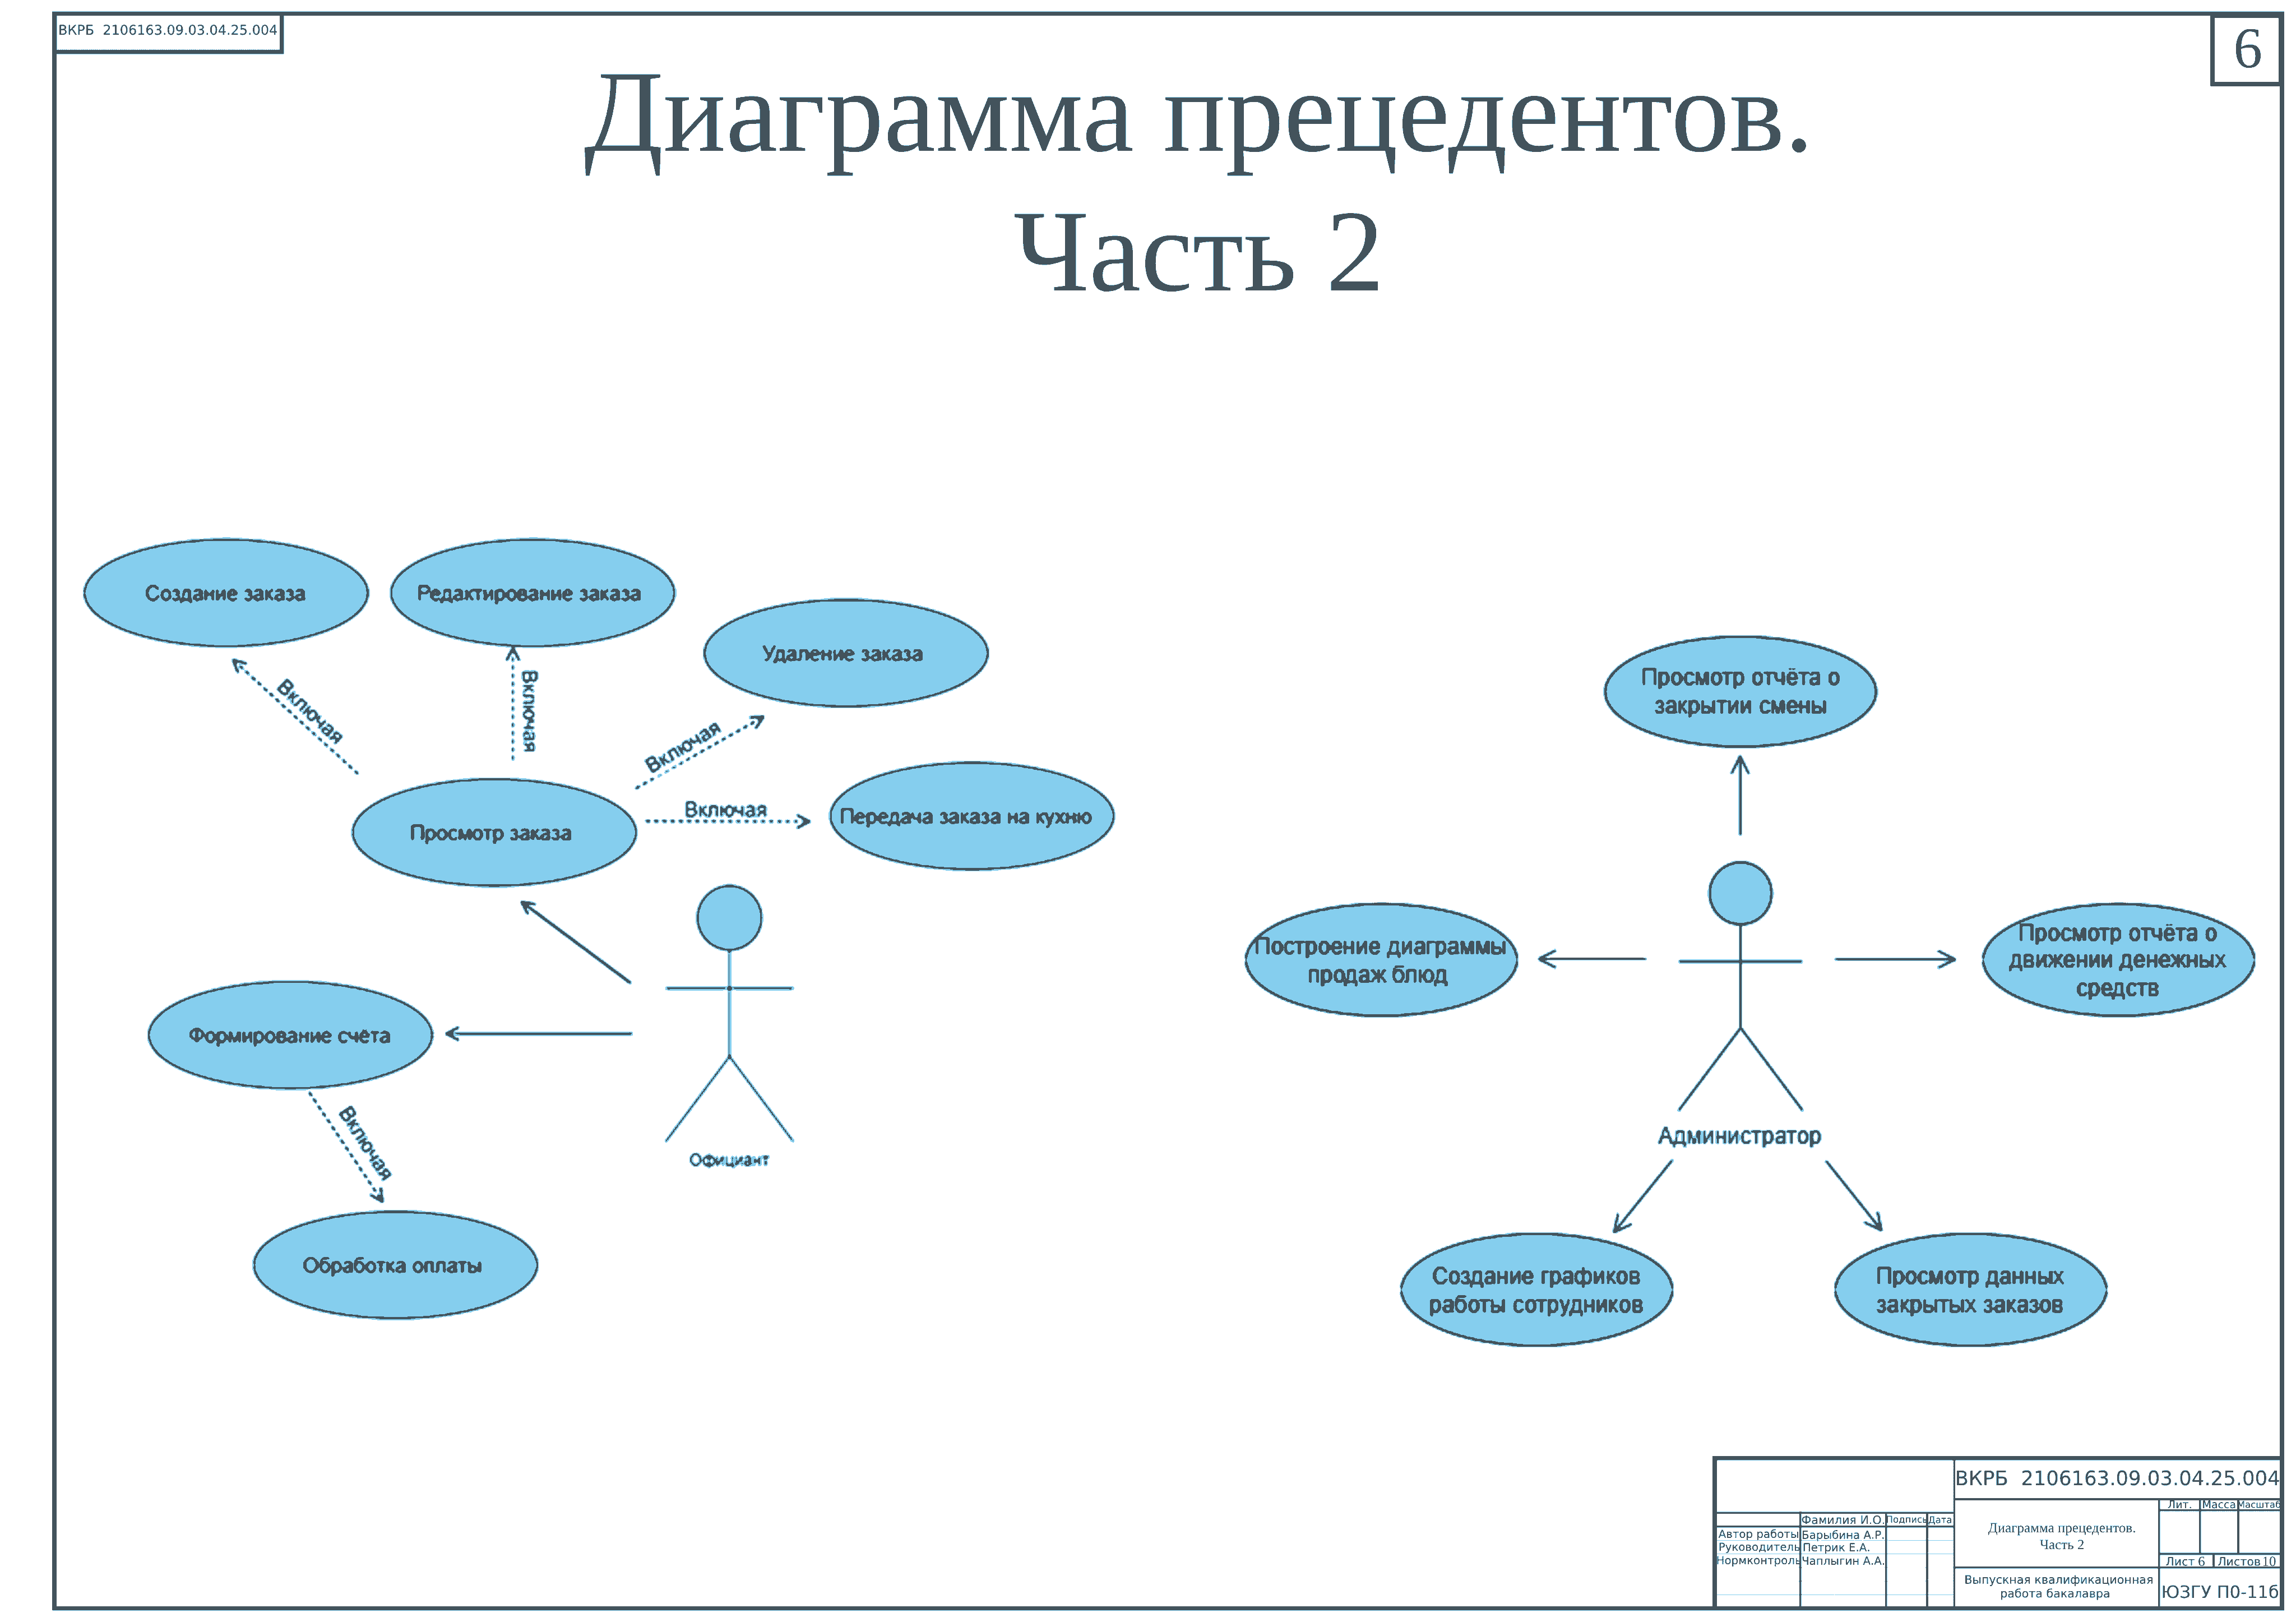
\includegraphics[width=0.84\linewidth]{precedent2.png}
	\заголовок{Диаграмма прецедентов. Часть 2}
	\label{pl6:image}      
\end{плакат}

\begin{плакат}
    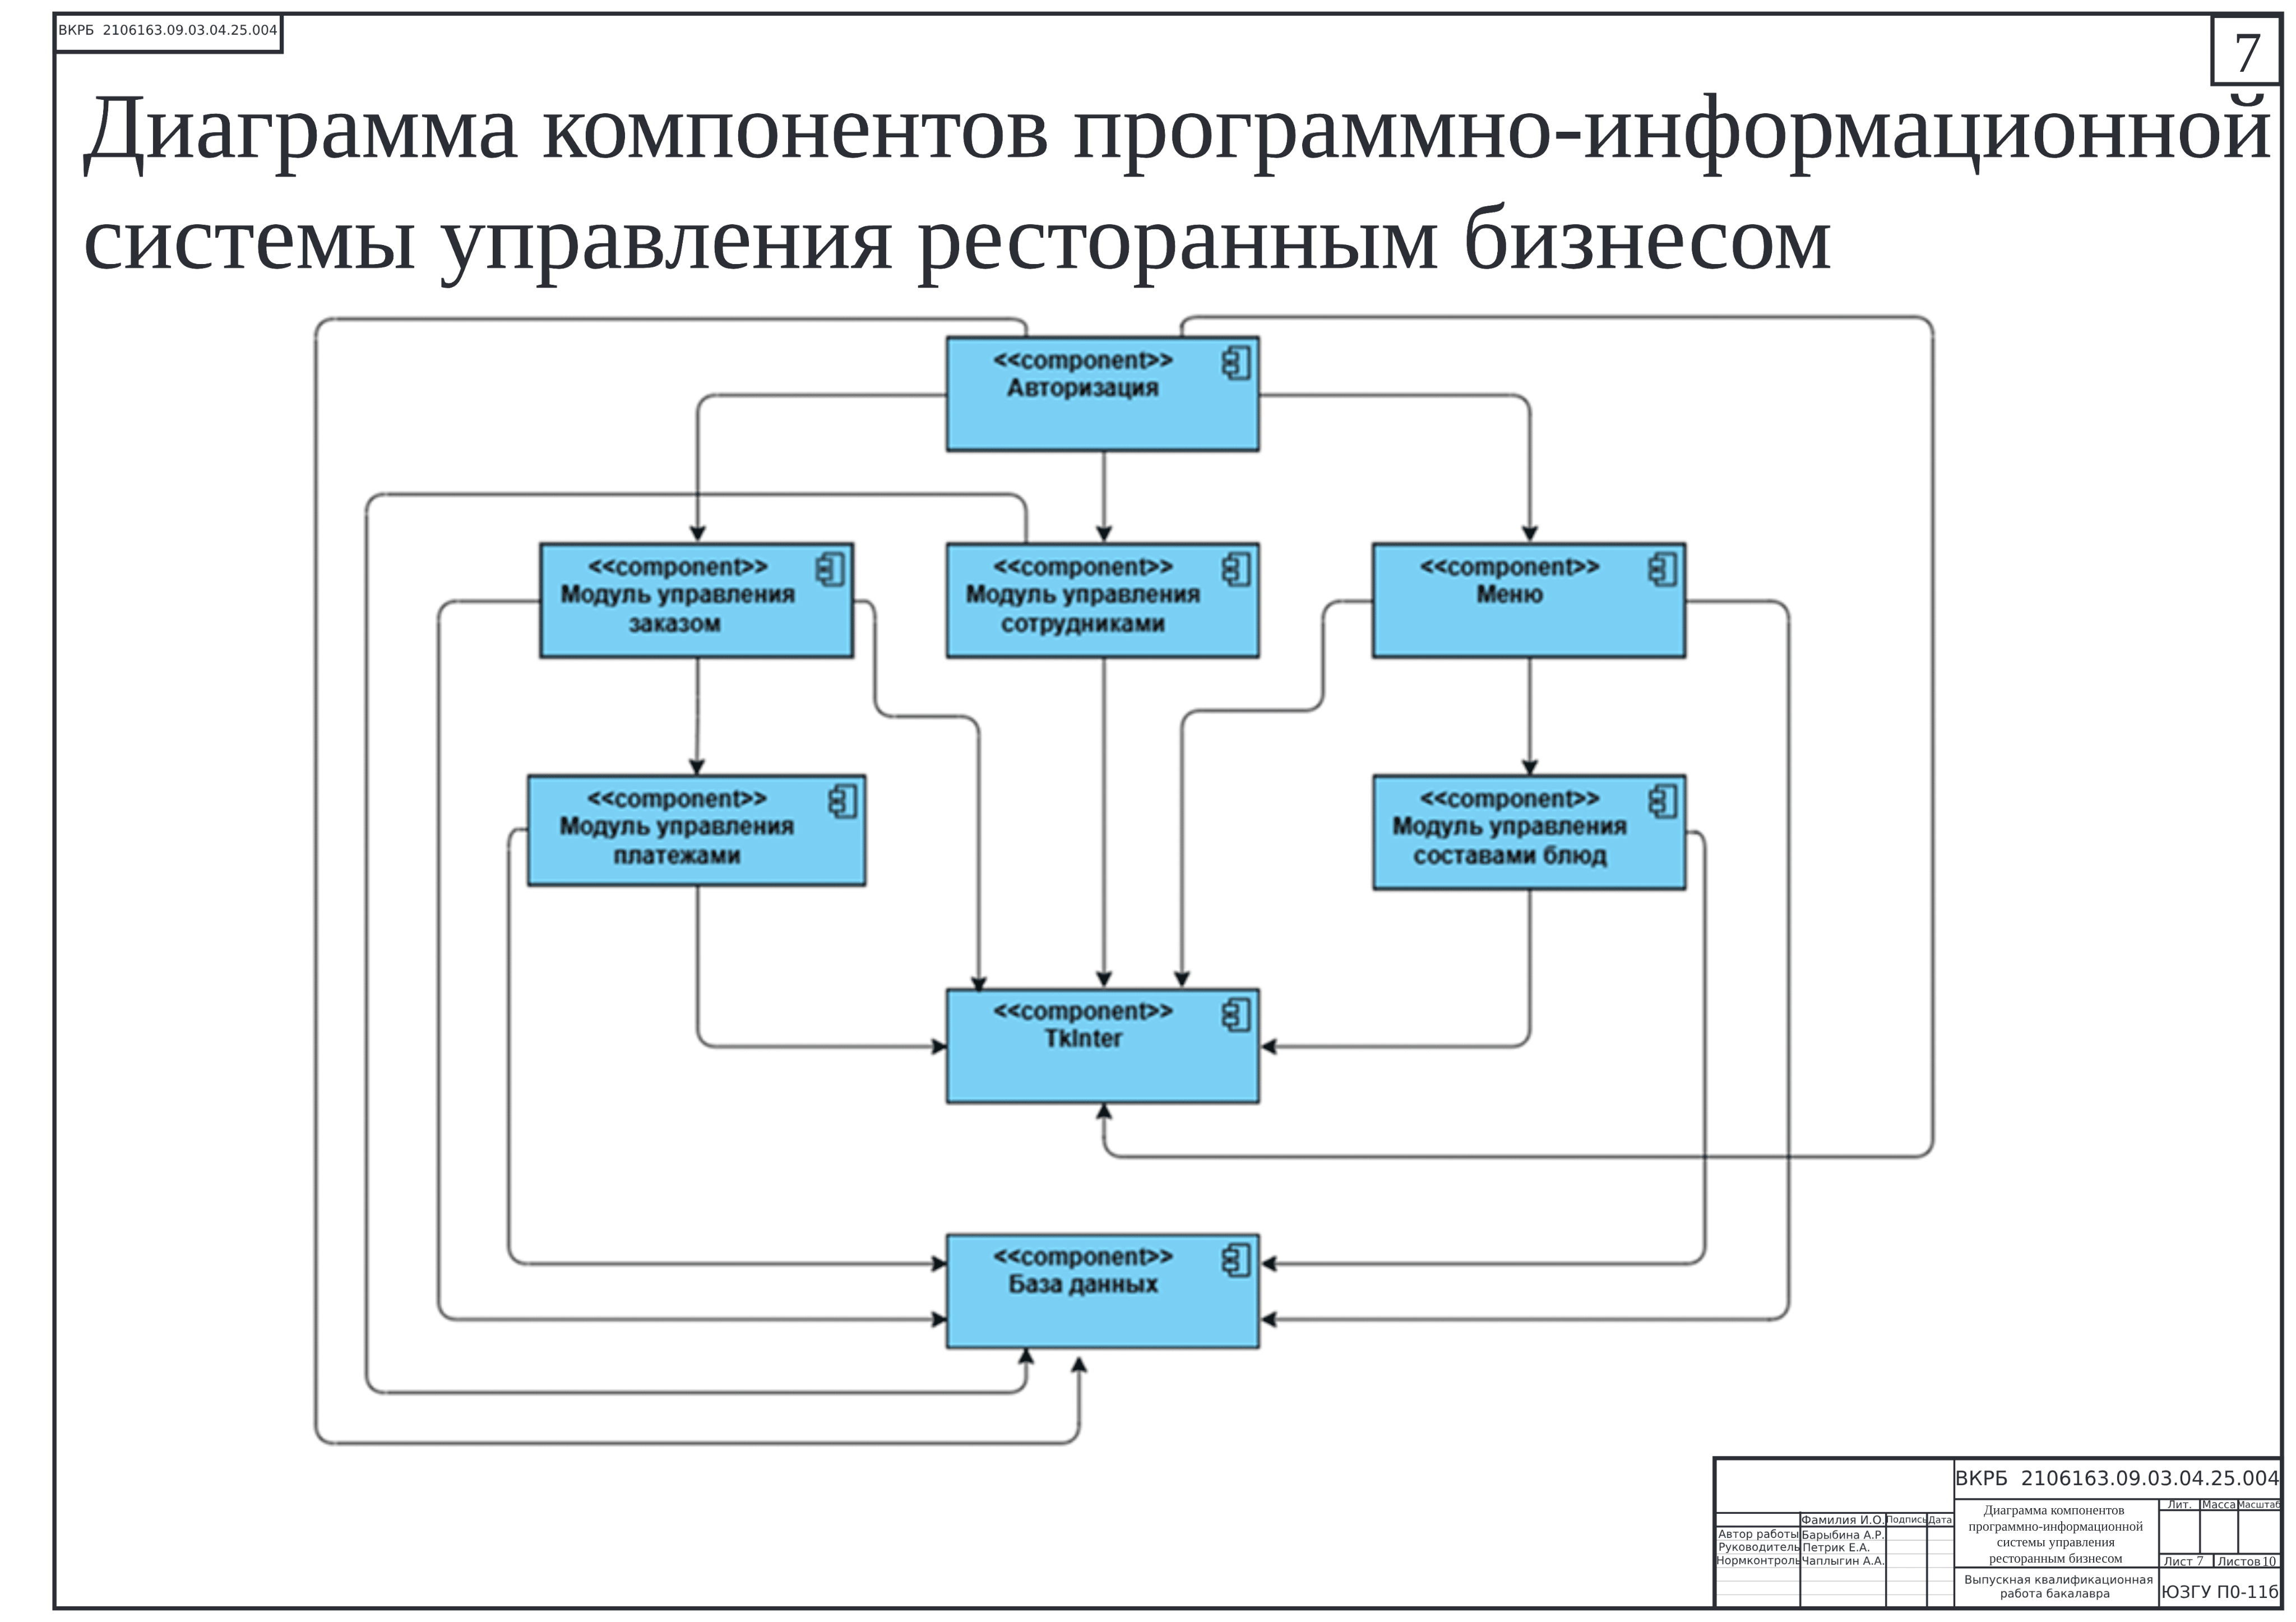
\includegraphics[width=0.84\linewidth]{components.png}
    \заголовок{Диаграмма компонентов программно-информационной системы управления ресторанным бизнесом}
    \label{pl7:image}      
\end{плакат}

\begin{плакат}
	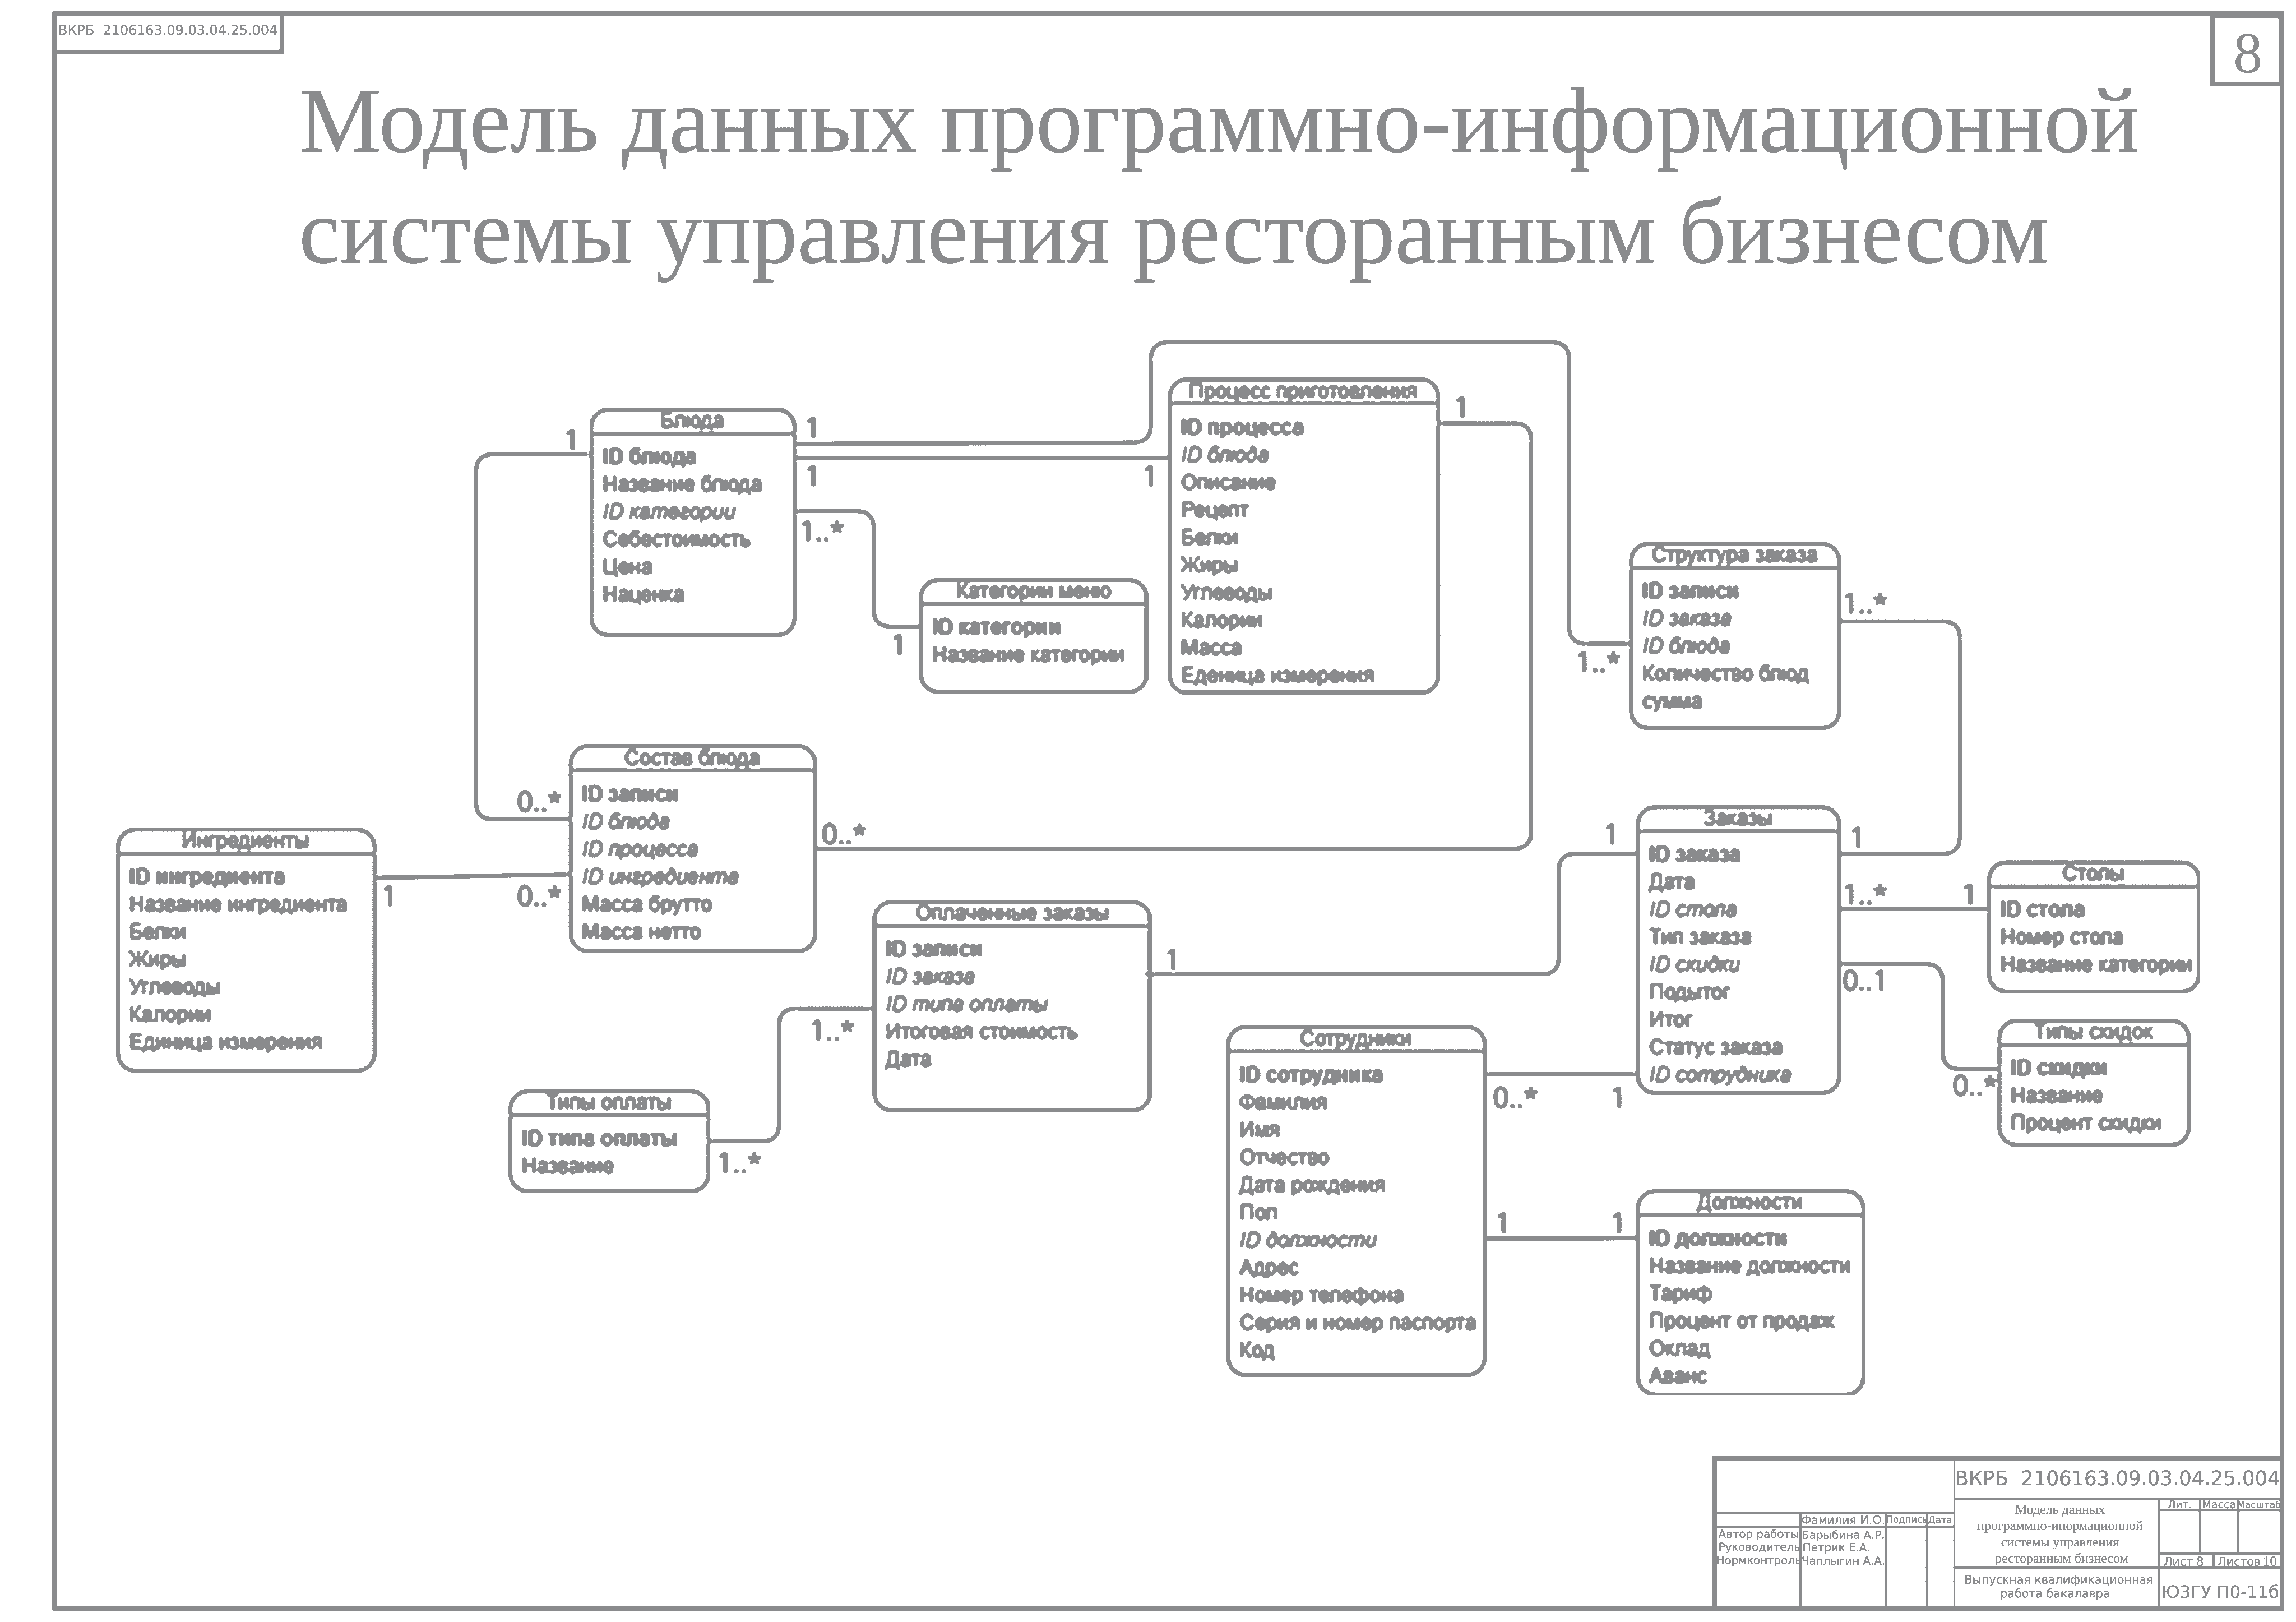
\includegraphics[width=0.84\linewidth]{erdiagramma.png}
	\заголовок{Модель данных программно-информационной системы управления ресторанным бизнесом}
	\label{pl8:image}      
\end{плакат}

\begin{плакат}
	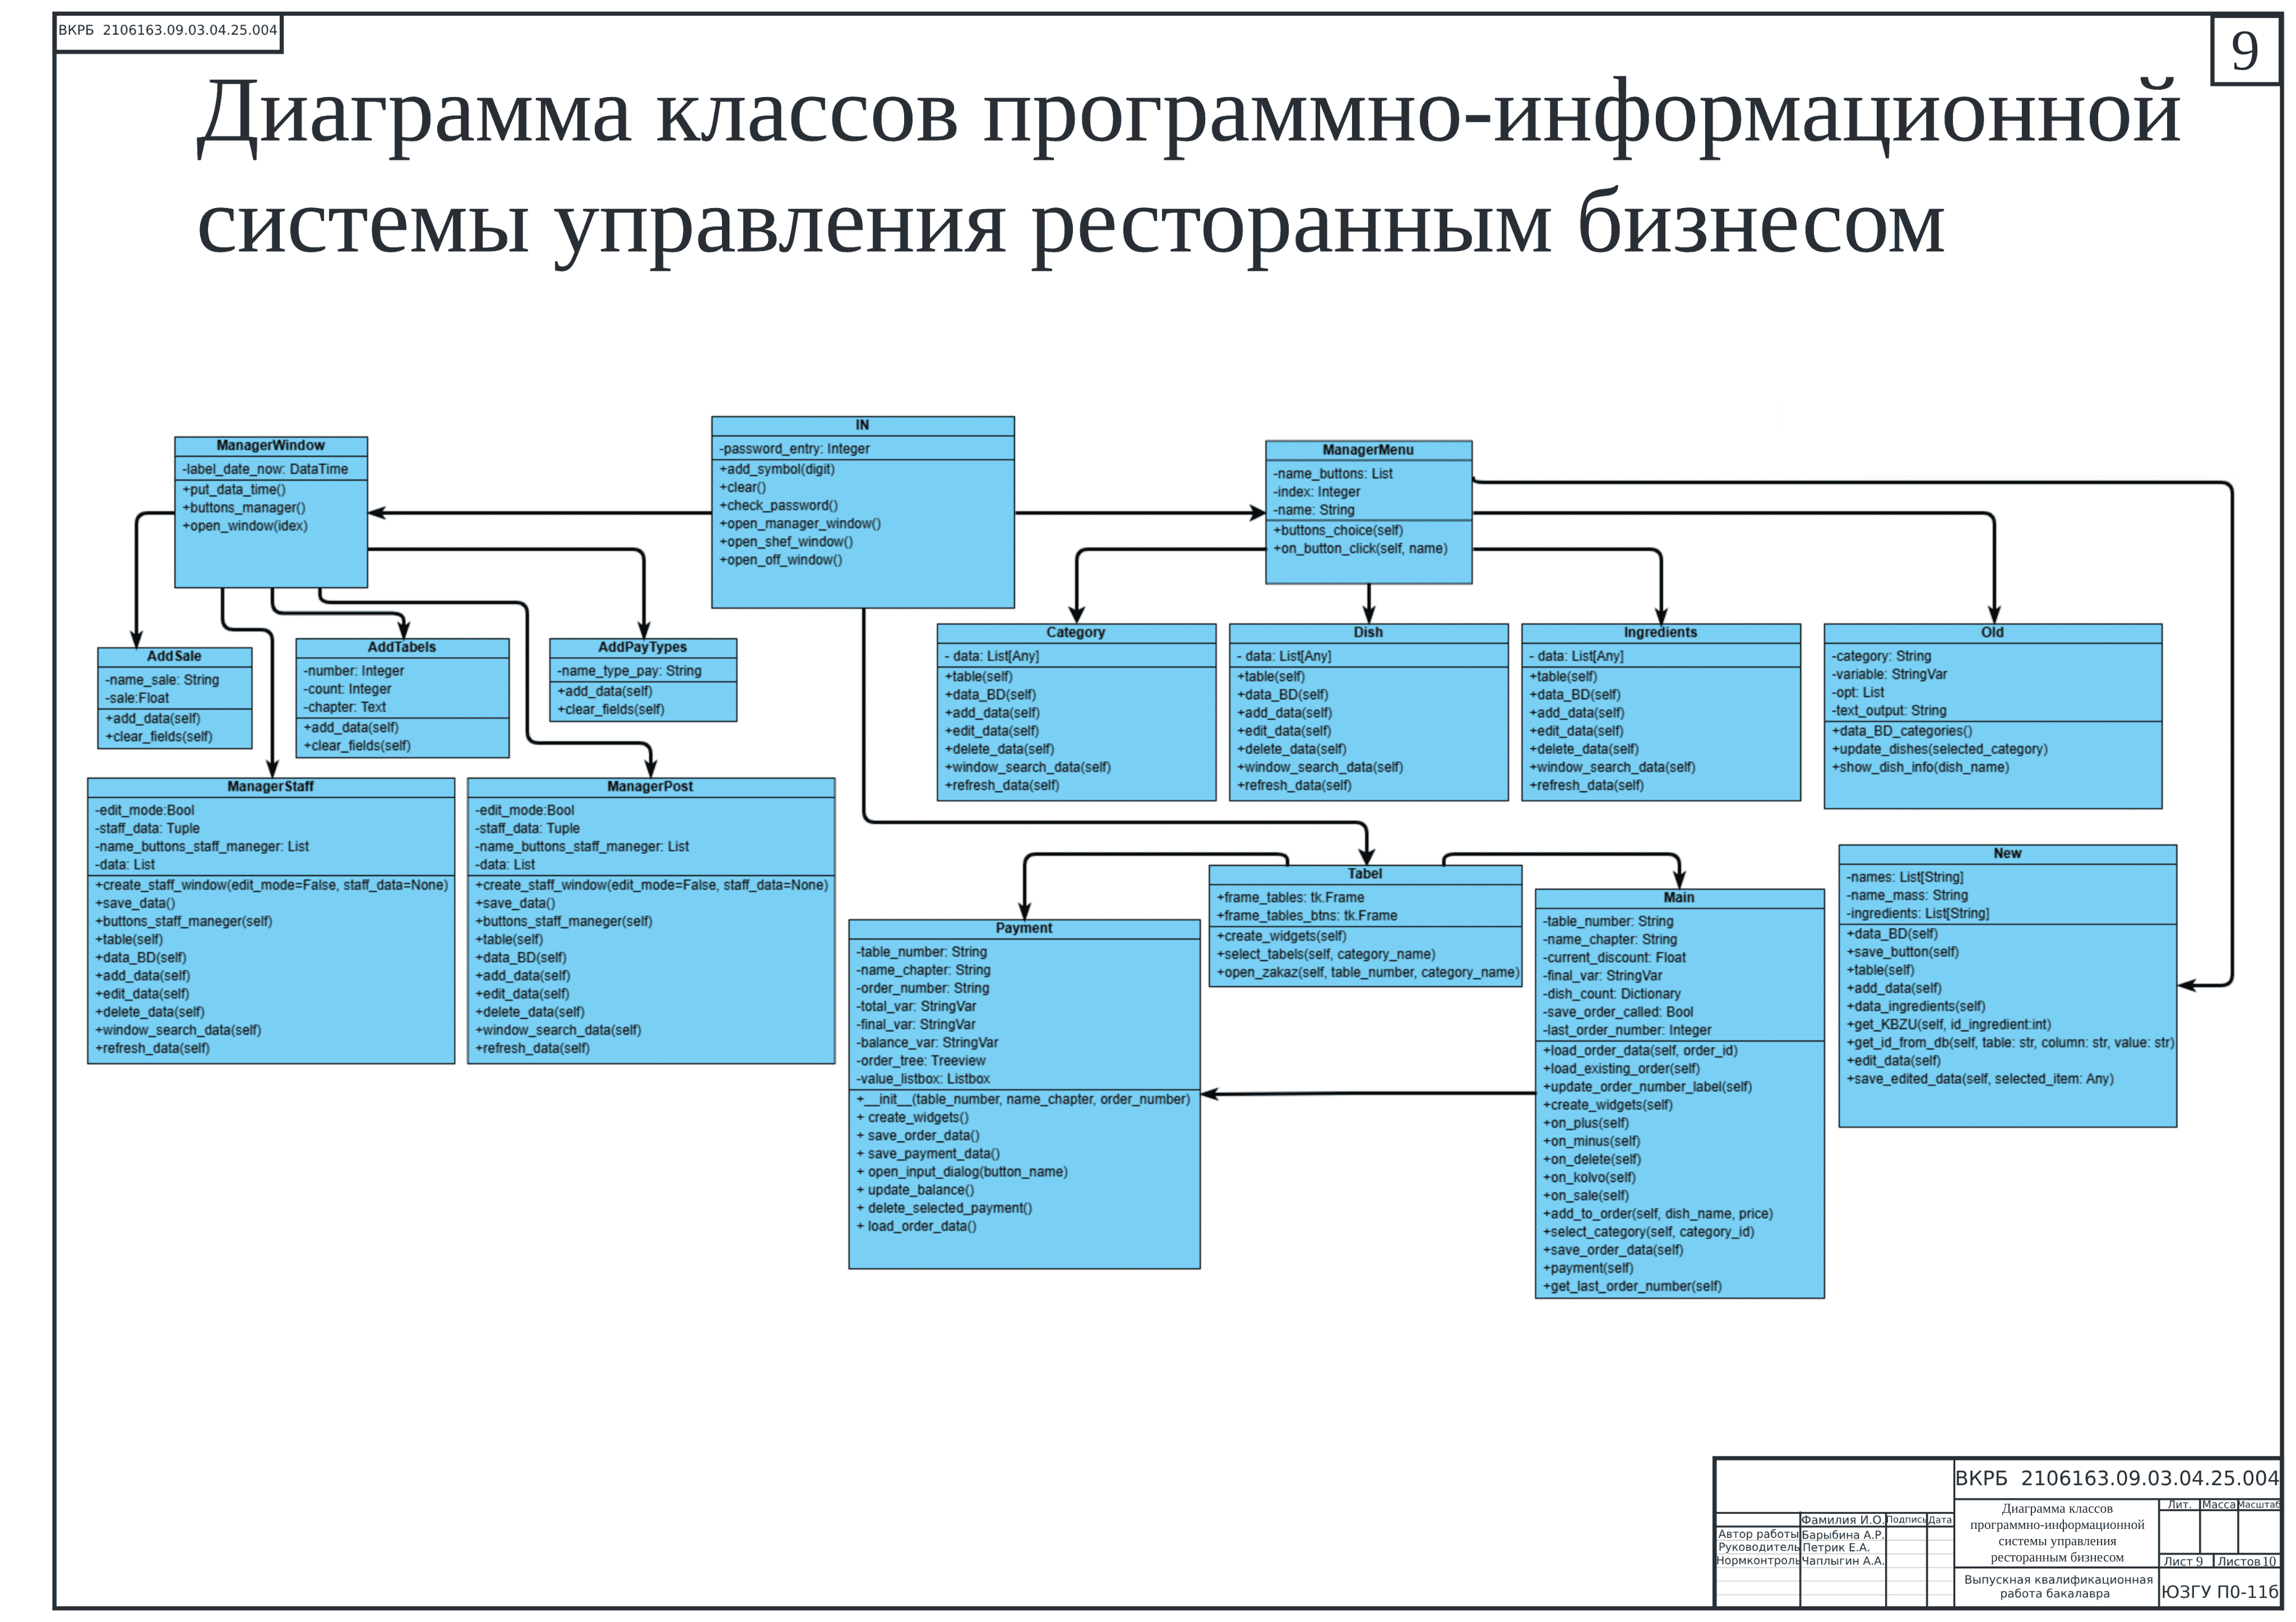
\includegraphics[width=0.84\linewidth]{classdiagramma.png}
	\заголовок{Диаграмма классов программно-информационной системы управления ресторанным бизнесом}
	\label{pl9:image}      
\end{плакат}

\begin{плакат}
	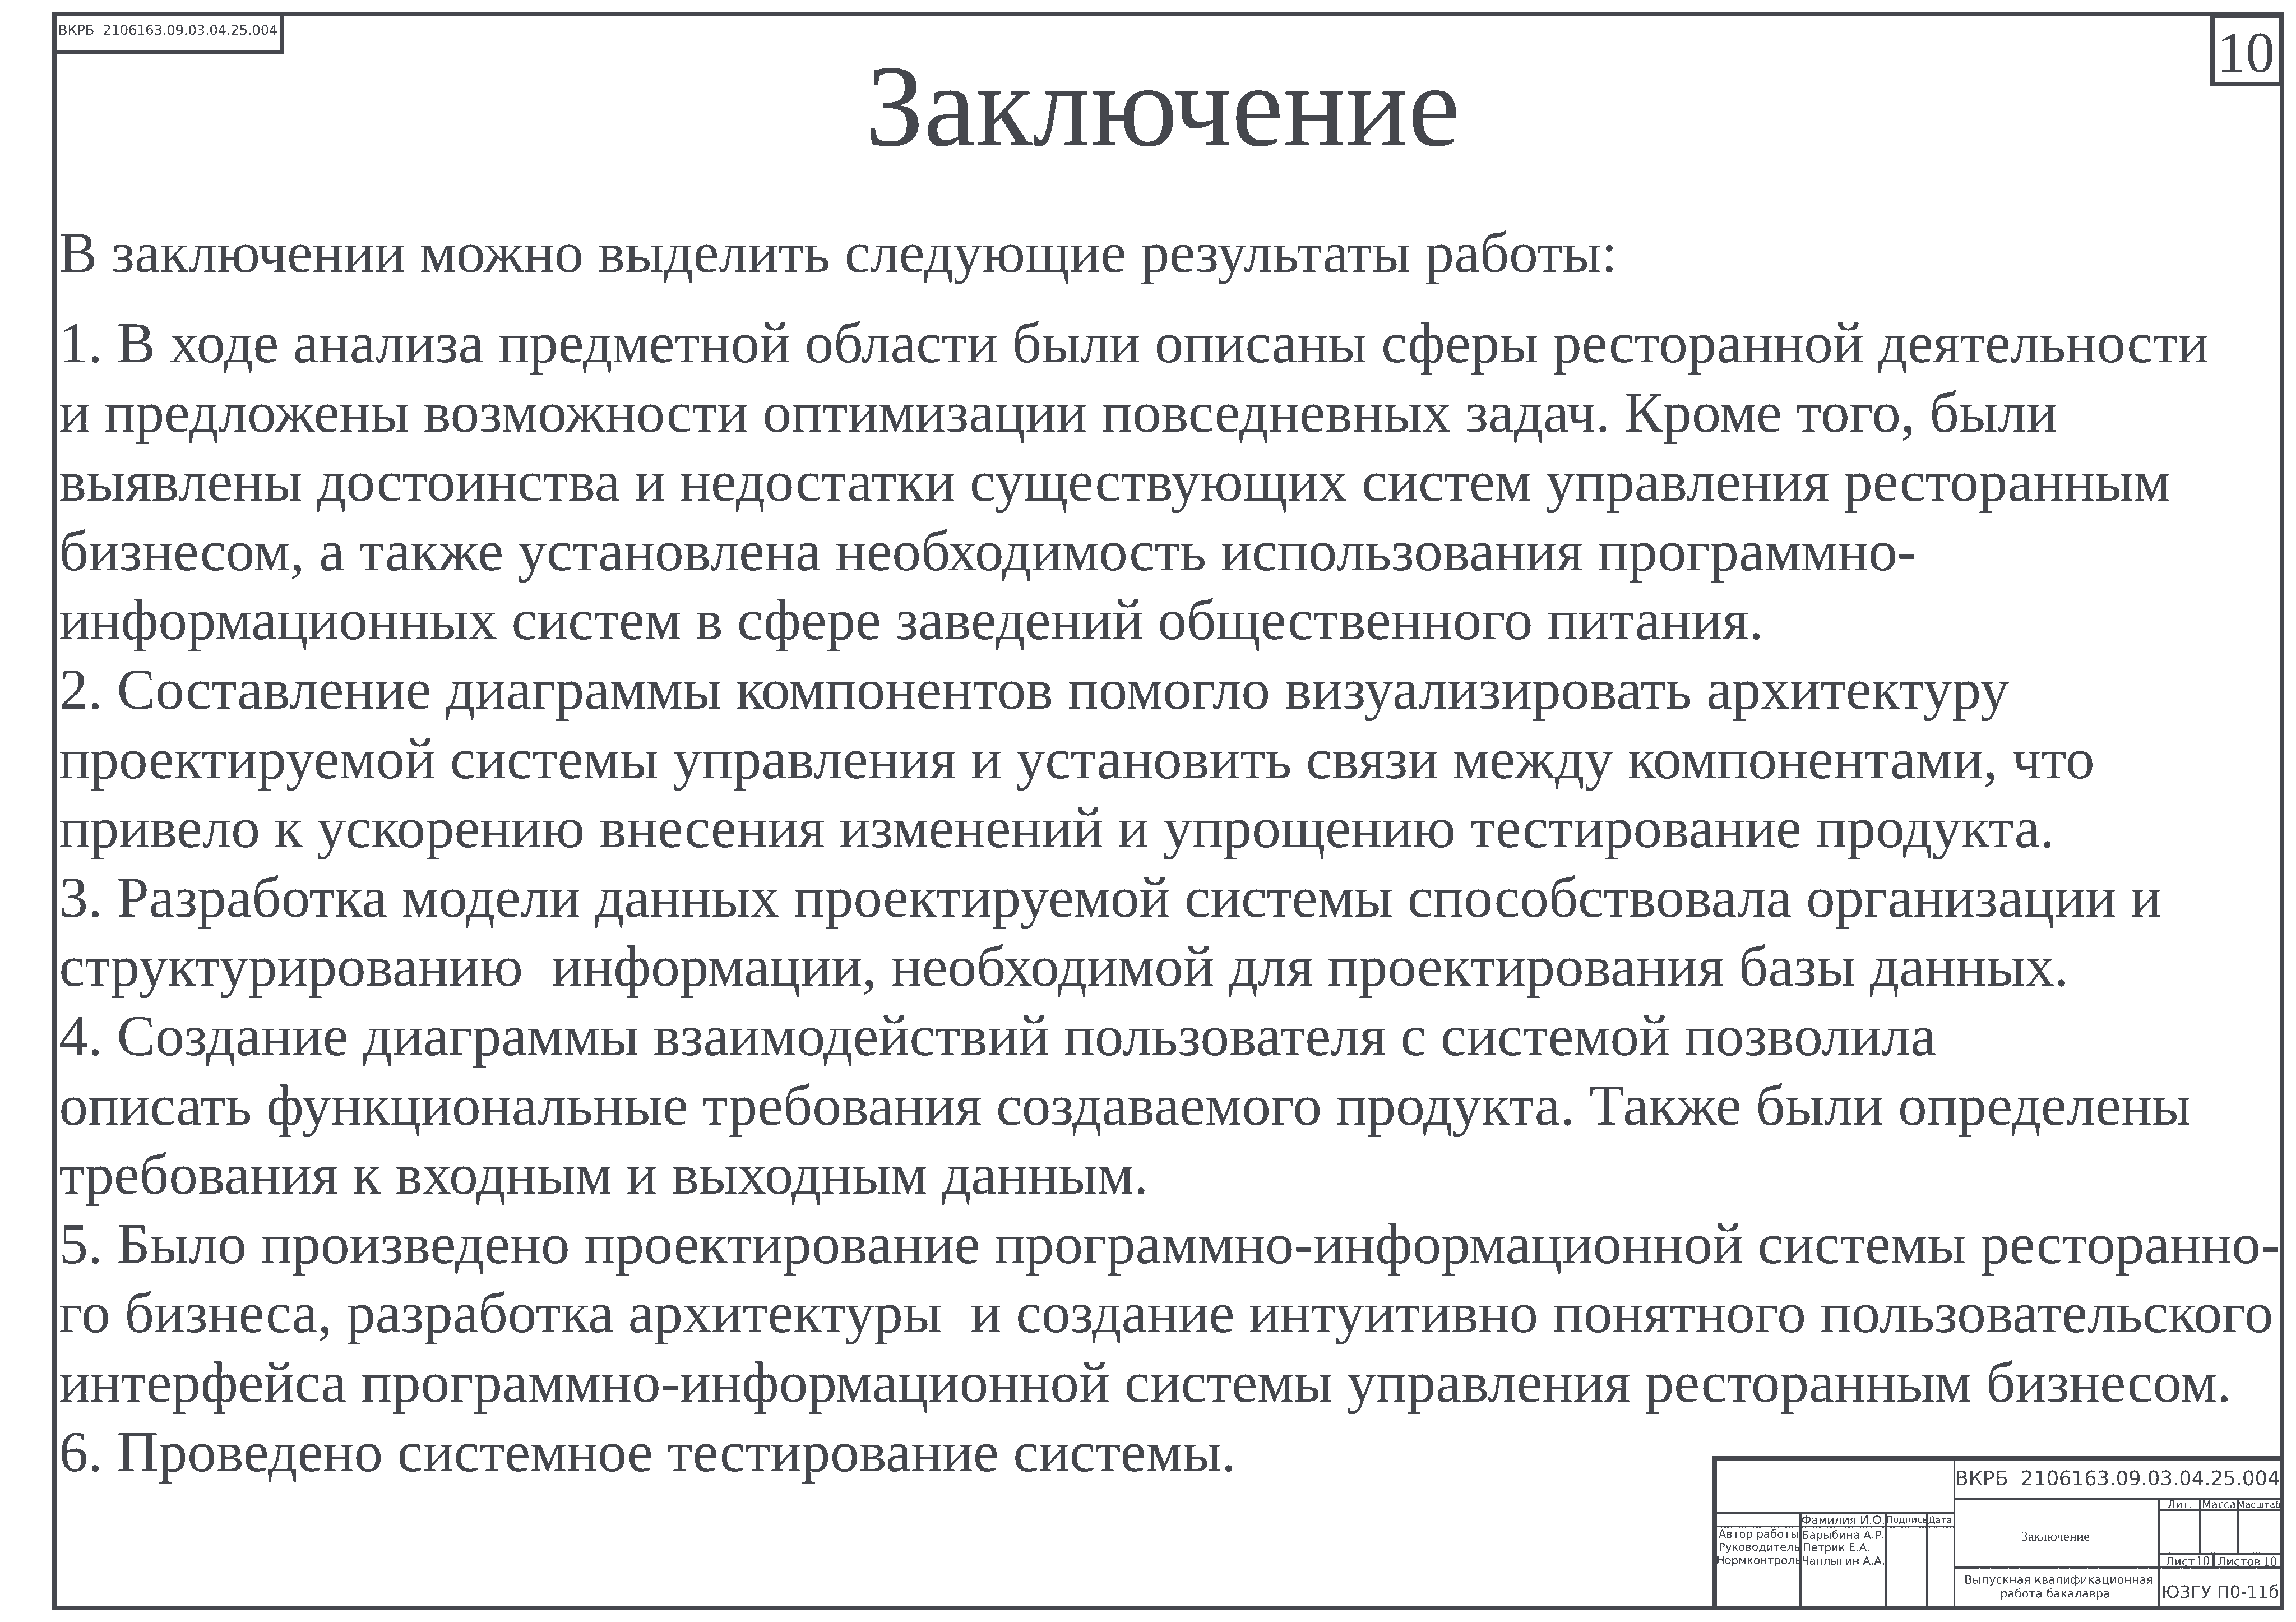
\includegraphics[width=0.84\linewidth]{end.png}
	\заголовок{Заключение}
	\label{pl10:image}      
\end{плакат}

\end{landscape}
